\documentclass[12pt]{article}
\usepackage{amsmath,amssymb}
\textheight 240mm
\textwidth  170mm
\oddsidemargin  0mm
\evensidemargin 0mm
\topmargin -20mm

\usepackage[utf8]{inputenc}
\usepackage{graphicx}
\usepackage{float}
\usepackage{titling}
\usepackage{geometry}
\usepackage{color}

\geometry{ a4paper,
	left=30mm,
	right=30mm,
	top=20mm,
}

\addtolength{\headheight}{0.2pt}
%\setlength{\droptitle}{-8em}

\title{Music Genre Classification}
\author{Abhijit Suresh, Paria Rezaeinia, Sahana Sadogopan}

\begin{document}
	\maketitle

\section{Introduction}
Music genre classification is the task of classifying the given audio signal into its corresponding categorical description (a.k.a. genre). It has been a very challenging task in the field of music information retrieval (MIR) and widely used for digital music service and internet radio. Music applications such as Shazam identify a song based on a part of the song. The goal of this project is to design a classifier that listens to a song and finds the genre of the song. 

The data set we are using for this project is the data set from the website of the 5th International Conference on Music Information Retrieval (ISMIR2004), and it is available in Pulse Coded Modulation (PCM). There are a total of 729 songs. The number of songs in each genre is as follows:
\begin{itemize}
	\item Classical: 320 songs
	\item Electronics: 115 songs
	\item Jazz-blues: 26 songs
	\item Metal-punk: 45 songs
	\item Rock-pop: 101 songs
	\item World: 122 songs
\end{itemize}
The goal of this project is to train a classifier on this data that can classify any song into these 6 different genres. We have explored several approaches to this problem. In order to train and test data, we use 10-fold cross validation. Therefore, 90\% of the songs are being used for training the classifier and 10\% of the songs for testing of the classifier.

Our approach to this problem is consisted of 3 main components; dimensionality reduction, defining distance in the new space and statistical learning. We discuss the dimensionality reduction techniques in section \ref{dr}. Section \ref{sec:dist} talks about the different distance metrics we explored. Section \ref{sec:stat} explains the statistical learning methods we have used to classify the data. In section \ref{sec:exp} we represent the results of our approach and finally in section \ref{sec:disc} we talk about the final results and possible future works to improve our results.

\section{Dimensionality Reduction}\label{dr}
%_________________________________________________________________
For analysis and training of our data we need to initially sample the songs . After the sampling of the given data set  ,the dimension of the data set is too large to classify them into different genre. When the dimension is enormously huge the data becomes sparse as the volume increase. This is known as the curse for dimensionality. Hence a Dimensionality reduction on the sampled dataset has to be performed to classify it genre. As the dimensionality is reduced we can use different clasiification methods. There is a certain limit to which dimensionality can be reduced without loosing important data. Johnson Lindestrauss Therom provides us with the limit to which the dimension can be reduced.
Johnson Lindestrauss states that considering n points in space of dimension $R^n$  where d is really large. The Dimension of my space can be reduced to $$k=o(log n)/\epsilon^2$$
The mutual distance between the pair of points is within the factor of $1\pm \epsilon$. This is the minimum dimension to which the data set can be reduced without major data lost.By using this theorem we use a $dxn$ matrice which maps the poins from $R^n$ space to a lower dimension of $dxn$ .
when we apply Johnson Lindestrauss to our current data set of 729 songs sample in space , we get that the minimum dimension to which we can reduce the dimensionality is 79.
%_________________________________________________________________
\subsection{mfcc}
The First dimensionality reduction technqiue that we used in MFCC (Mel Frequency Cepstrum Coefficient) \cite{logmfcc}. In Mel Frequency Ceptrum the frequency bands are equally spaced in mel space which is approximated by the human auditory system clearly,this frequency system allows for better representation of song.
The MFCC coefficient follows a sequence of steps through which the coefficients are found.
The diagram below shows the sequence of steps in the generation of the mfcc coefficient.
\begin{figure}[H]
\center
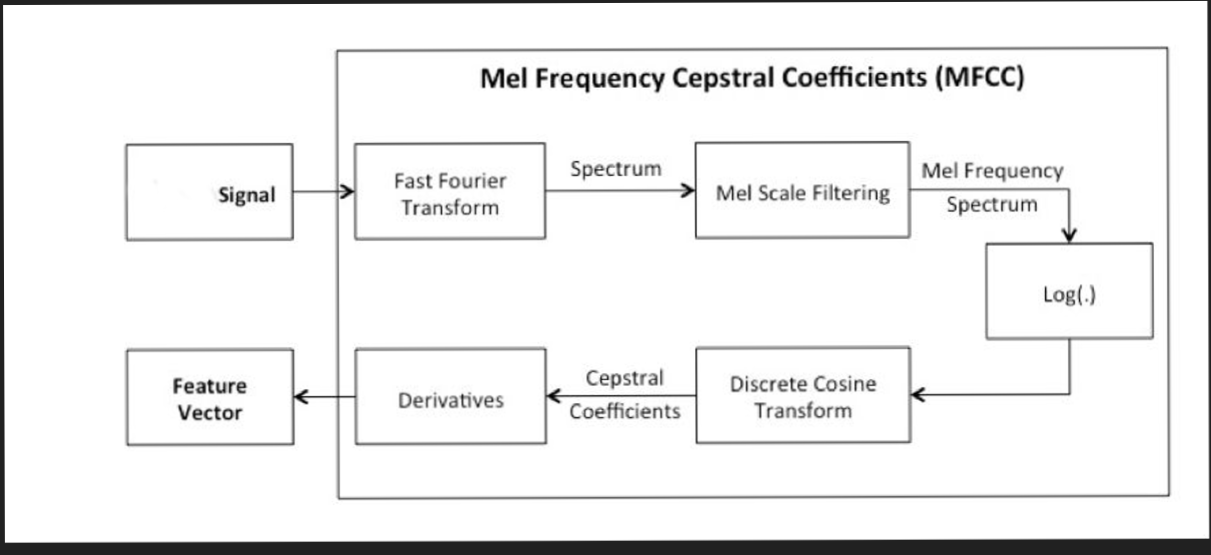
\includegraphics [scale=0.5]{mfcc.png}
\caption{mfcc algorithm}
\end{figure}
In the above figure as shown after the signal is sampled , first the fourier transformation is performed and the spectrum obtained is passed through the Mel Scale Filter. The output that we obtain is the Mel Frequency spectrum.
The log of the result is taken and a discrete Fourier transform is applied to the signal the result of this is the Mel Frequency Coefficient.
After performing the MFCC we have the signal saperated into different slots and each slots contain a the feature vectors. As suggested by johnson Lindestrauss we have taken 79 features per slot.The number of slots changes acoording to the length of the song.
\subsection{PCA}
PCA(Principal Component Analysis) is a kind of linear transformation to perform dimensionality reduction of subspace. PCA reduces the dimension by projecting the d dimensional data set onto k dimensional subspace where $k<d$ \cite{holand}. The data that we got from MFC is passed on to PCA. The dimensionality reduction even after MFCC is quite huge to calculate the distance and classify them into different genre.
PCA calculates direction in which variance of the data is maximum. There are few steps followed to calculate the direction of the space.
\begin{itemize}
  \item The data obtained from MFCC is normalised first
  \item The mean of the normalised data is put in a matrix and the mean value for all the rows are obtained.
  \item The variance of the data from MFCC is calculated.
  \item The Eigen values and Eigen vectors are calculated from the covariance matrix.
  \item The Eigen vectors are sorted in descending order in order to get the k largest eigen values.A new matrix is formed from the dominant eigen values.
  \item Then the data set is project on this new subspace and the feature vector are organised.
\end{itemize}
\subsection{Content based similarity}
Beth and Ariel \cite{logan} presents a novel approach to compare songs based on their corresponding audio content. For each song in the dataset, they create a song signature. The song signature is generated based on k-means clustering of spectral features. The algorithm is summarized in figure (\ref{content}) below.

\begin{figure}[h]\label{content}
\center
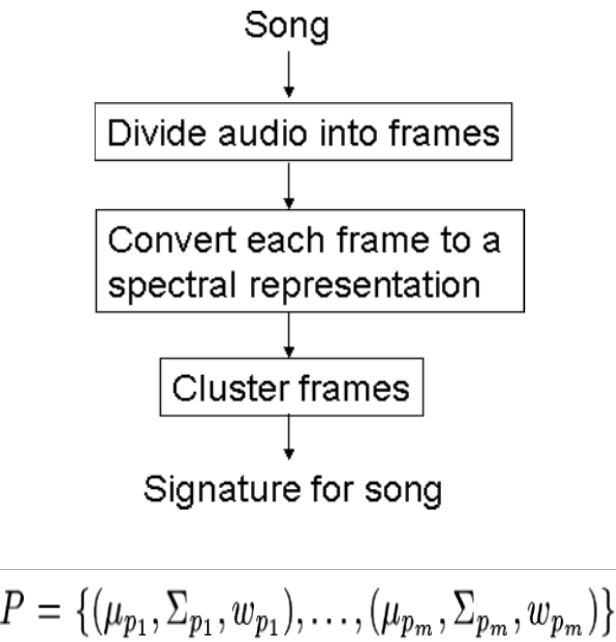
\includegraphics{fig1.png}
\caption{Content based similarity method}
\end{figure}

The first setup is to divide the audio into frames. Then, each frame is converted into its corresponding spectral representation. In order to generate the spectral representation we make use of mfcc algorithm which is explained in the previous sub section. The number of cepstrum coefficients was calculated based on the Johnson-Lindenstrauss lemma.

\subsubsection{Johnson-Lindenstrauss}
The idea behind Johnson-Lindenstrauss lemma is that points in high-dimensional space can be projected onto low dimensional space while preserving the distance between the points \cite{dasgupta}. For a given dataset, the minimum number of dimension required to preserve the distance between the points is given by the formula $$ n > 8 * ln(m) * \epsilon ^ 2 $$ where $\epsion$ is a number between 0 and 1. For this project we have $$ n > 77$$ and hence the number of cepstrum coefficients that we have considered is 79.

\subsubsection{k-Means}
Once each frame is clustered into its corresponding we spectral representation, we cluster the frames using unsupervised k-Means clustering algorithm where the value of k is  fixed to 10. k-Means is a popular clustering algorithm used in data mining. It is often confused with k-nearest neighbour algorithm which makes use of supervised labels during the training phase in order to cluster the points. Given a set of n observations in a d dimensional space, k-Means aims to cluster the n dimension into k sets $S = {S_1,S_2,...S_k}$ where $ k \leq n$. The idea is to find the sum of distance functions of each point in the cluster to the K center. The equation is given by (\ref{kmeans}):

\begin{figure}[h]\label{kmeans}
\center
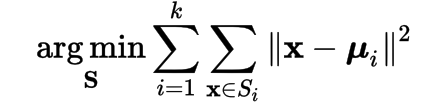
\includegraphics{fig2.png}
\caption{k-Means}
\end{figure}

\paragraph{}
After identifying the clusters, the mean, covariance and weight is calculated for each cluster. This set of values forms the signature of the song. This signature is used in order to compare two songs.

\subsection{Modified Gaussian Mixture} \textcolor{red}{Paria}

\section{Distance Metrics}\label{sec:dist}
This section provides the different types of distance metrics that we used in our project. Distance metric is used to quantify the distance between two different songs in the song space. However, the distance metric is valid only on a low-dimensional sub space due to curse of dimensionality. For example: Consider a hypersphere. As the number of dimension increases the volume of hypersphere tends to zero. This phenomenon is also called as concentration of measure. In such a concentrated space euclidean or any type of distance is not meaningful. Hence, before calculating the distance we need to use dimension reduction as pre-processing step. The list of techniques that we experiment with for dimension reduction is discussed in the previous section (\ref{dr}).


\subsection{Minowski}
Minowski distance is considered as the generalization between euclidean distance and manhattan distance. This distance metric is used along with k-nearest neighbour for classification of points for songs which was reduced by content based similarity method. The reason why we used Minowski distance over other distance metric is based on experimentation. The distance between two n-dimensional point $ X = {x_1,x_2,...,x_n}$ and $ Y = {y_1,y_2,...,y_n} $ is calculated as:
\begin{figure}[h]\label{kmeans}
\center
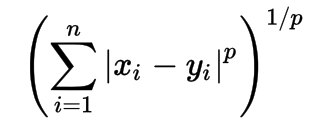
\includegraphics{fig3.png}
\caption{Minowski distance}
\end{figure}
\subsection{Earth Movers distance}
Earth Movers distance is the distance between two different probability distributions over a region D. This is the distance metric used to compare the distance between two songs using the signatures generated by the content similarity method. In the field of mathematics, it is also known as wasserstein metric. Informally, it is defined as the cost of turning one pile of dirt into another. EMD value is given by the formula:
\begin{figure}[h]\label{emd}
\center
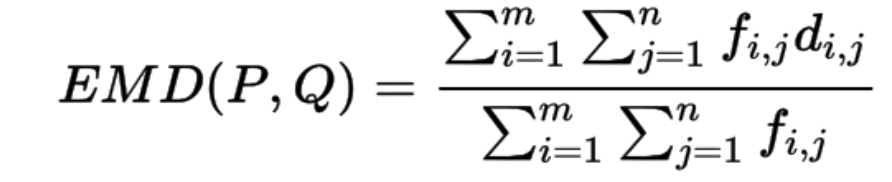
\includegraphics[scale=0.5]{emd.png}
\caption{EMD}
\end{figure}
\paragraph{}
where $f_{i,j}$ is the flow between cluster i and j and is calculated based on weight of the cluster. $d_{i,j}$ is the ground distance between the clusters. In this case euclidean distance is used as the ground distance. The numerator is denoted by the work and is normalized by the flow. The distance matrix generated by EMD is as follows:
\begin{figure}[H]\label{emd_dist}
\center
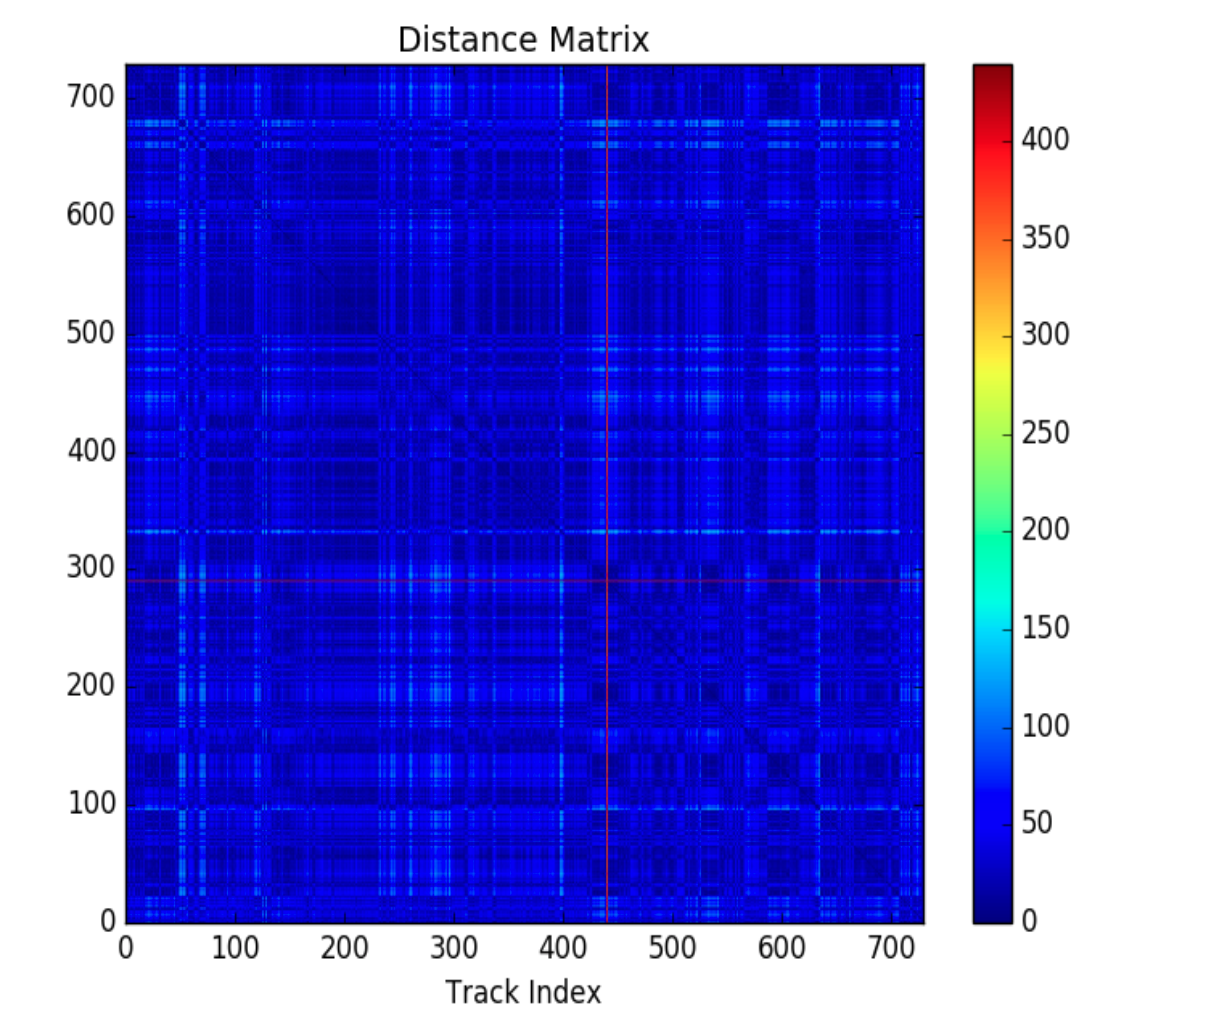
\includegraphics[scale=0.8]{emd_dist.png}
\caption{Distance matrix using EMD}
\end{figure}
In order visualize the distance matrix as scatter plot, we use multidimensional scaling (MDS). MDS is a means of visualizing the level of individual classes of a dataset. In this case, the classes refer to the different genres. Based on the scatter plot we find that there are no linearly separable regions to separate once class from another. The classes seem to be correlated to each other. Hence, linear classification algorithms such as linear regression will not perform as expected.
\begin{figure}[H]\label{emd_scatter}
\center
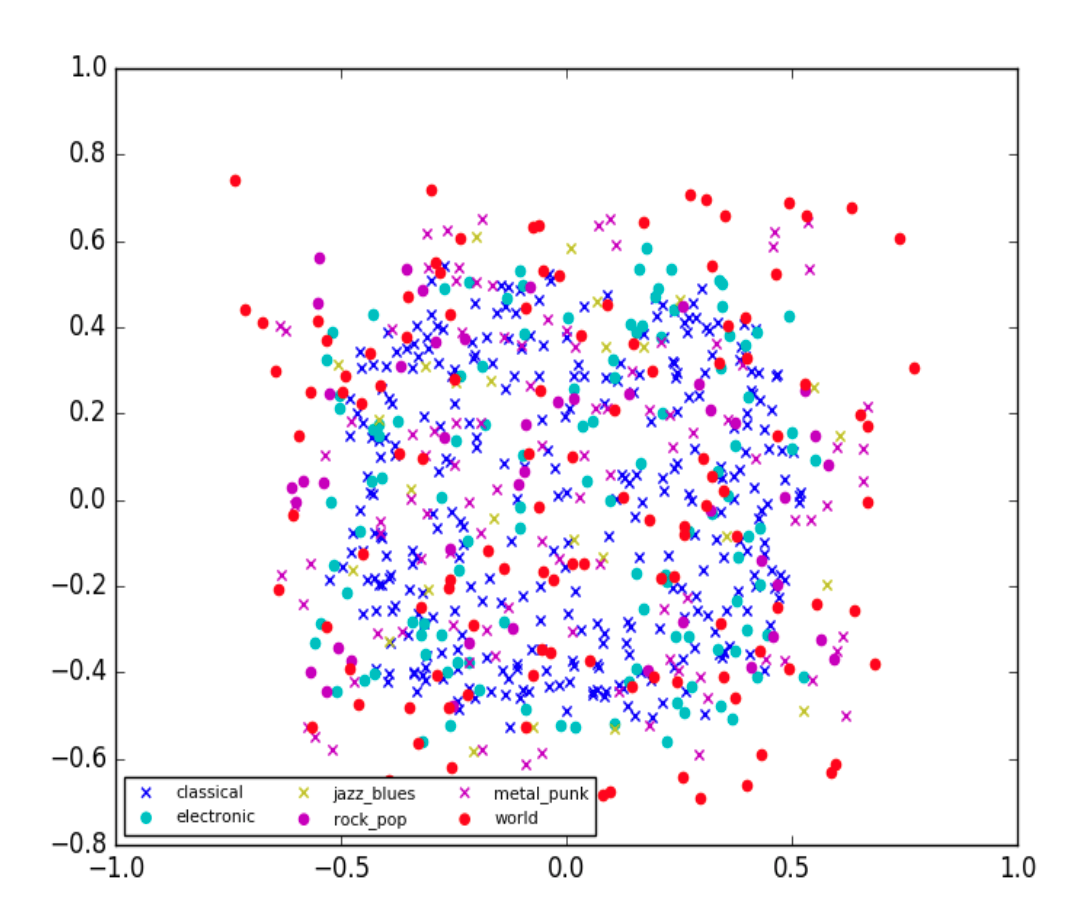
\includegraphics[scale=0.8]{emd_scatter.png}
\caption{Scatter Plot}
\end{figure}

\subsection{Euclidean distance}
Euclidean distance also known as $l^2$-norm is a common measure of distance between two points in n-dimension space. Euclidean norm is simply the magnitude of the vector. This norm is very simple to calculate. Therefore, in our experiments we start with the Euclidean norm and if the result did not provide a good performance, then we test other distance metrics relevant to the data. In addition to be simple to calculate, Euclidean distance has a good performance in a braod range of settings. The following picture represents the distance matrix using modified Guassian mixture model and Euclidean distance.
\begin{figure}[H]\label{distMat30}
	\centering
	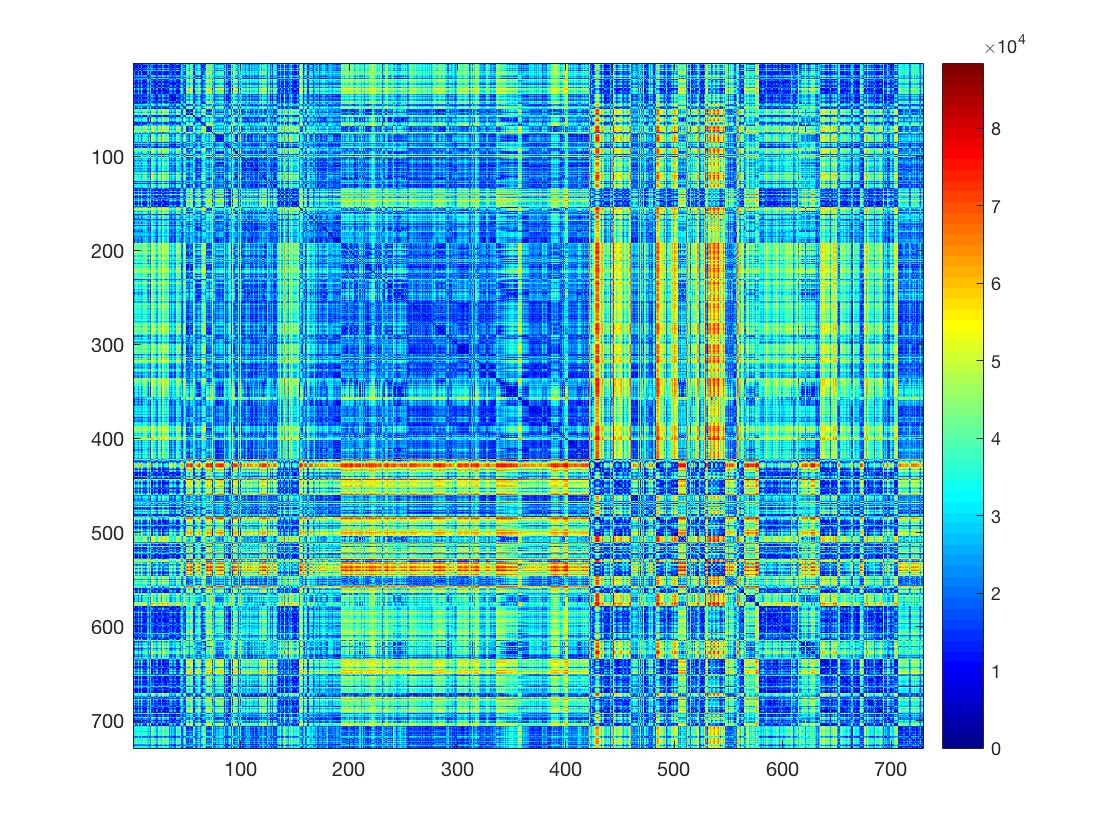
\includegraphics[width=1\linewidth]{distMat30.jpg}
	\caption{Euclidean distance matrix for modifed Gaussian mixture model}
\end{figure}
\subsection{Kullback-Leibler Divergence}
Kullback-Leibler divergence (KL) distance is a measure of distance between two given probability distributions. If $P$ and $Q$ are two probability distributions, then the KL-divergence can be written as:

\begin{equation}\label{KLdist}
D_{KL}(P||Q) = H(P,Q) - H(P)
\end{equation}
In this equation, $H(P,Q)$ is the cross entropy of the two probability distributions, and $H(P)$ is the entropy of $P$. \\
For discrete probability distributions, the KL-divergence is given as the following equation:
\begin{equation}\label{KLdist}
D_{KL}(P||Q) = \sum_i P(i) log \frac{P(i)}{Q(i)}
\end{equation}
Therefore, the KL distance is a measure of the information loss in estimating probability distribution $P$ with probability distribution $Q$. As you can see from equation (\ref{KLdist}) this distance is not a symmetric distance. The following figure shows the distance matrix for our data set using modified Gaussian mixture model and KL-divergence as distance metric.
\begin{figure}[H]\label{KLDiv}
	\centering
	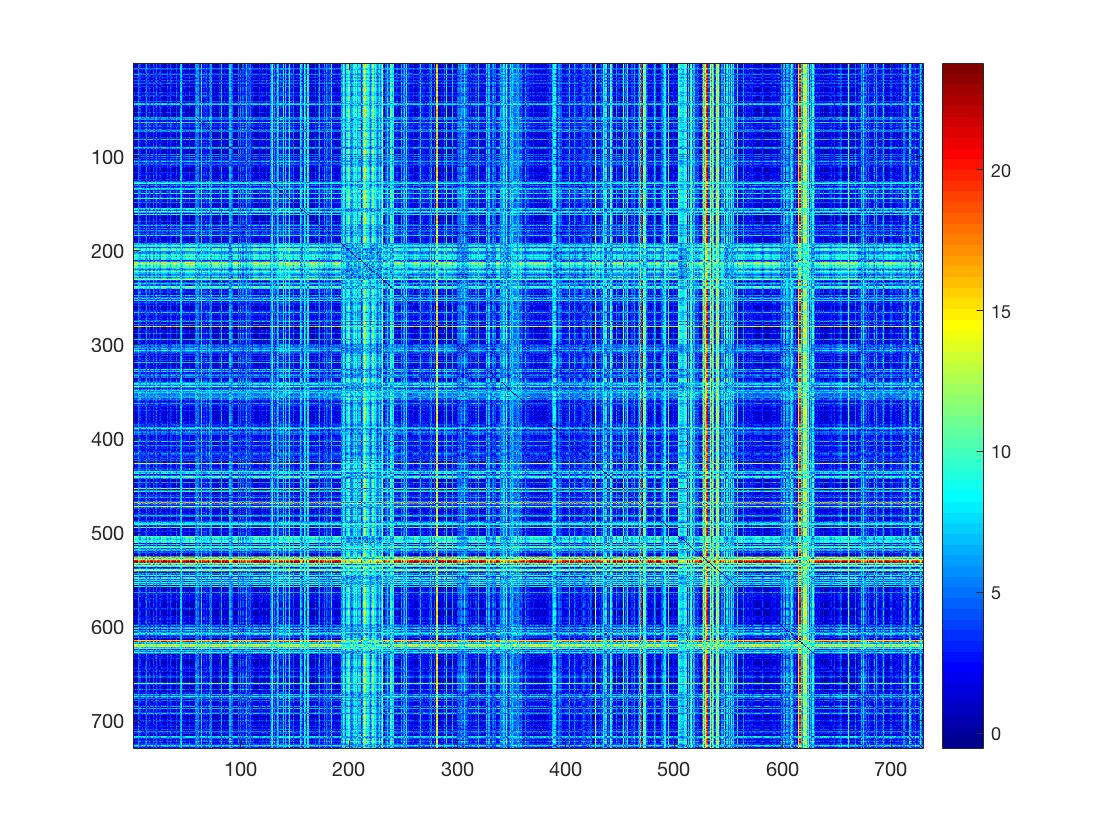
\includegraphics[width=1\linewidth]{KLDiv.jpg}
	\caption{KL distance matrix}
\end{figure}
In this distance matrix, we can see the genre classes that we have as squares around the main diagonal of the matrix. But, there is also small distance across multiple genres. For example, we can see small distance between the songs in the classical genre and the songs in the world genre.
\section{Statistical learning}\label{sec:stat}
In previous sections we discussed the projection of audio files into lower dimensional space. And we introduced the measure of distances we use to represent the distance between the new representations of the audio files. The next step is to build the classifier to these information for genre classification. We have implemented three classifiers that we explain here.
\subsection{k-Nearest Neighbors}
One of the common algorithms for classifying multi-class data is k-nearest neighbors (kNN) \cite{li}. This algorithm simply finds the k closest data points to the testing point and determines which class owns the majority of points among these points. Therefore, the label for the testing data point would be the label of the majority of k closest data points.
The following figure represents the kNN algorithm for $k = 3$. There are 2 classes in this example represented with blue and red color. The testing point is the black circle and because 2 out of 3 closest neighbors are in blue, the classifier will assign it to the blue class.
\begin{figure}[H]\label{kNN}
	\centering
	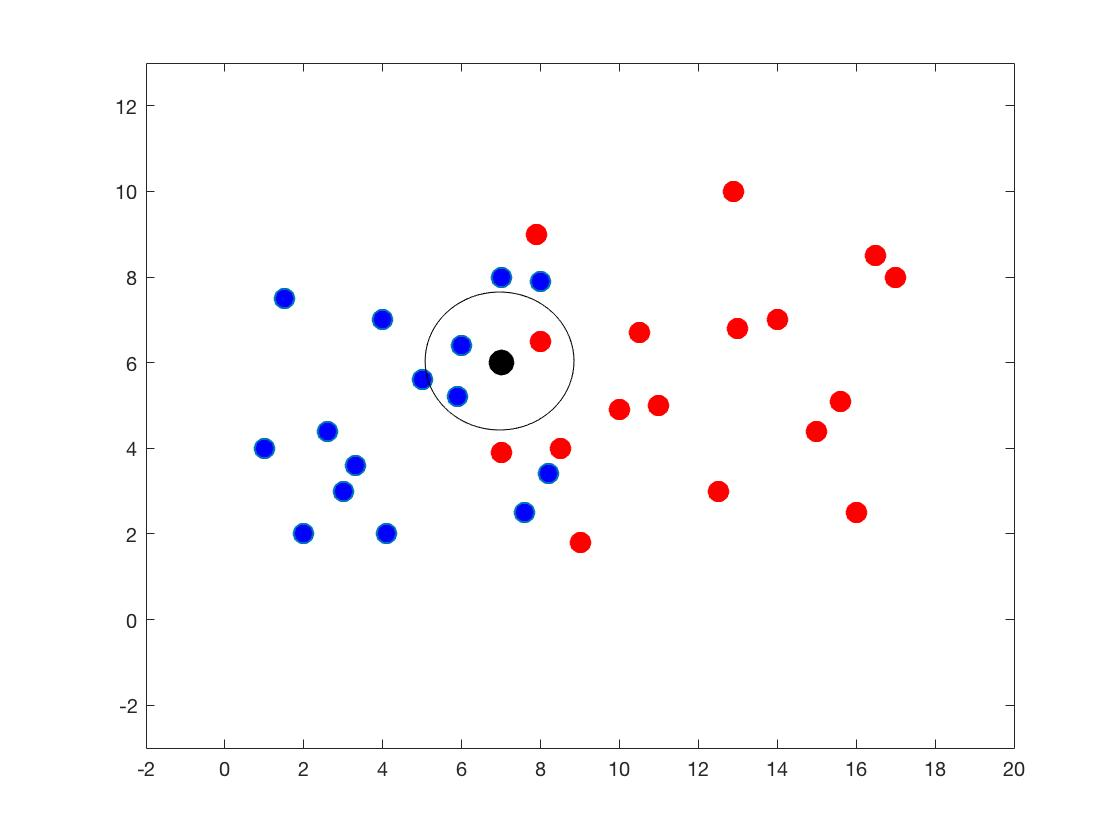
\includegraphics[width=.8\linewidth]{kNN.jpg}
	\caption{k-nearest neighbors}
\end{figure}

The kNN algorithm do not provide a good performance if the training data points are not distributed uniformly among the classes. In this project we are using 729 songs, which contains 320 classical, 115 electronics, 26 jazz-blues, 45 metal-punk, 101 rock-pop and 122 world genre. Therefore, 43\% of all songs are classical and so, in any neighborhood it is more probable to have more data points from classical genre than any other genre. On the other hand, there are 26 jazz-blues songs which is less than 4\%. Thus, the probability of classifying a song as a jazz-blues song using kNN classifier is very low. Therefore, the kNN does not provide a good performance for the data set that we are using. The major error using kNN is classifying non-classical songs as classical songs. It also has a 100\% error for jazz-blues genre. In order to overcome this problem we have modified the kNN algorithm to take into account the frequency of each genre.

\subsection{Modified-kNN}
As we mentioned in the previous section, in order to make kNN classifier more powerful we introduced the modified kNN algorithm. In the modified-kNN classifier, we normalize the number of neighbors in each genre by the frequency of that genre (the number of training points in that genre divided by the total number of training points) in the training data. This classifier can be considered a special case of weighted-kNN, where the weights are the frequency of that genre. This algorithm improves are results for genres other than classical genre, but degrades the performance for the classical genre. And, the overall accuracy of the classifier increases.

\subsection{Neural Network}
Neural Network is a machine learning algorithm that is inspired by the method the brain functions when a problem is given. The large number of neurons have so many connections that it computes many combinations and gives us the most accurate answer.
As in the human brain as the signal goes back and forth , similarly in the neural network used of classification we have used the feedforward-back propagation.
The neural network basically consist of three different layers
\begin{itemize}
  \item Input Layer
  \item Hidden Layer
   \item Output Layer
\end{itemize}

Below Diagram shows a basic diagram showing the layers of a Neural Network
\begin{figure}[H]
\center
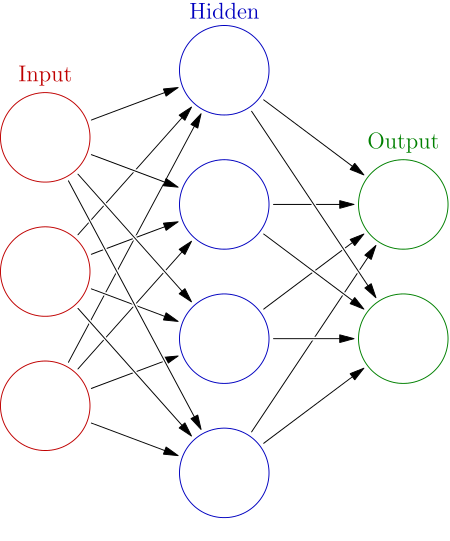
\includegraphics [scale=0.5]{ann.png}
\caption{Sample Neural Network}
\end{figure}
The connections between the input Layer and the hidden layer have weights that are multiplied to each connection. The weights are selected as per Gaussian values i.e they are between 0 and 1.
The Hidden Layer also have an active function whcih could be any mathematical function. For our classification we have used Levenberg-Marquardt


The neural network has three contributing factor that changes the efficiency of the output.
\begin{itemize}
  \item Weights given to the connections
  \item Active Function of the hidden layer
   \item The Learning algorithm
   \end{itemize}
 The Back propagation method is the learning algorithm used, in this algorithm we calculate the error when the synoptic weights are chosen randomly and calculate back the weights. By this method the error is reduced by calculating back the synoptic weights.\\
 The neural network used in this project is shown below
 \begin{figure}[H]
\includegraphics [scale=0.5]{NeuralNetwork.png}
\end{figure}
The input given is 20 features for each song and this is passed to hidden layer that contains 10 neurons and finally classifies the input to 6 genres.

\section{Experiments}
%_________________________________________________________________
Describe the experiments, and include the confusion matrix. Discuss
the influence of the various parameters, and describe how the optimal
parameters were chosen. Include the computation time for your method.
The general idea for genre classification is first Dimensionality Reduction, finding the distance matrix and then classifying the genres.
Hence in this project we used various dimensionality reductions such as MFCC,PCA,Modified Gaussian Mixture Model and Content based similarity. Decreasing the dimension is a crucial in genre classification as it avoids dimensionality curse.
In this project we tried a different set of combinations of the dimensionality reduction,distance calculation and classification methods.
The distance matrix is calculated for all the methods.\\ 
The confusion matrix for all the methods are shown below. First is the result of the Signature method Dimensionality reduction for which the distance is calculated through Earth mover distance method and classified into genre using KNN Classification.
 \begin{figure}[H]
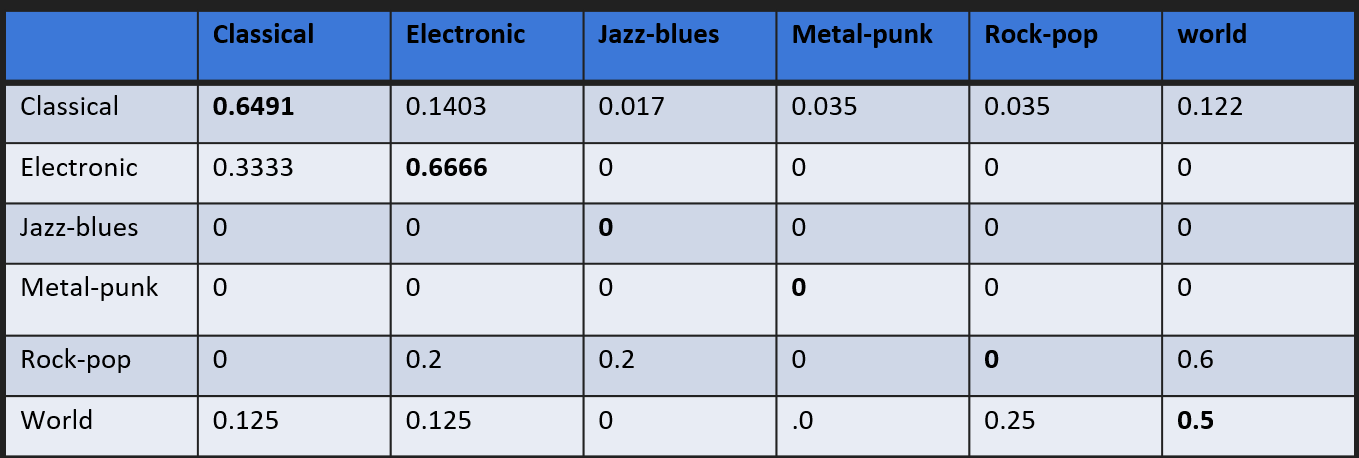
\includegraphics [scale=0.35]{results1.png}
\end{figure}
The average accuracy for this method was 54. \\
The second method that was performed was using Modified Gaussian mixture with euclidean distance and KNN classification.The efficiency obtained for this method is $52$.
\begin{figure}[H]
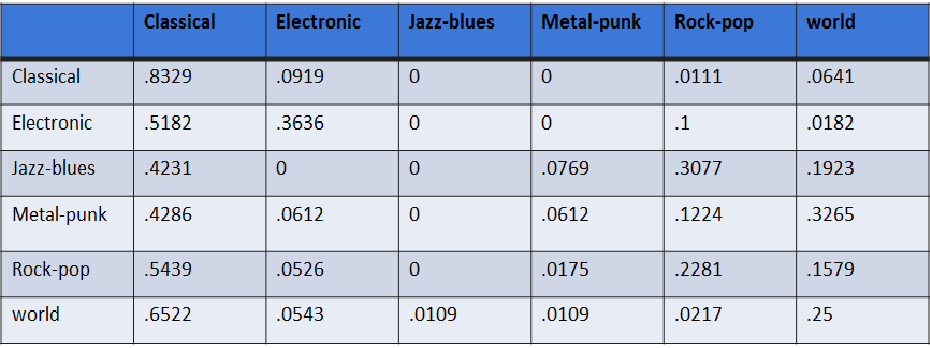
\includegraphics [scale=0.65]{result2.png}
\end{figure}
We tried increasing the dimension and performed the same methods as above we can say that the efficiency increases as the dimensions are increased. Below is the confusion matrix when d=50.
\begin{figure}[H]
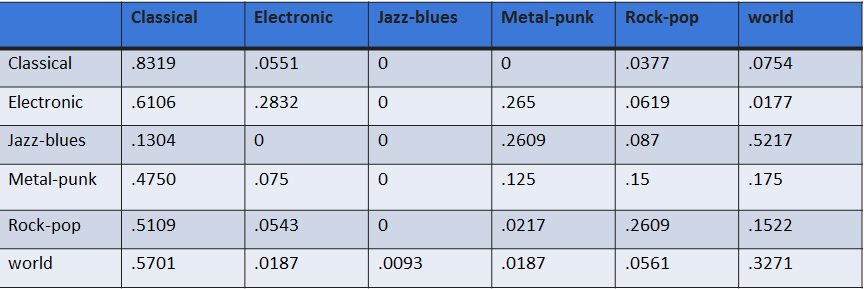
\includegraphics [scale=0.7]{result3.png}
\end{figure}
Next we changed the method by which the classification to obtain better classification of genre.Modified KNN method was used which gave better results as shown in the confusion matrix below.
\begin{figure}[H]
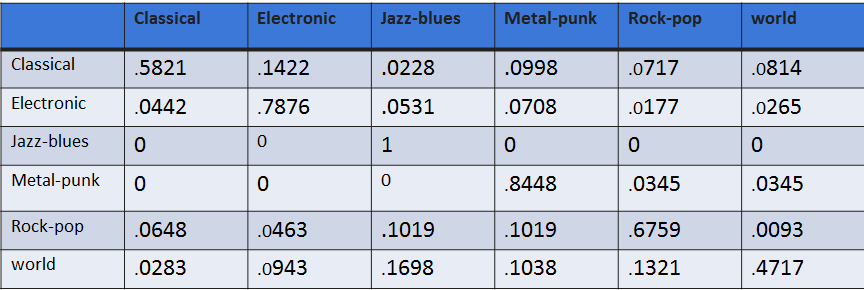
\includegraphics [scale=0.7]{result4.png}
\end{figure}
Finally the basic method of dimensionality reduction was implemented a(MFCC and PCA),euclidean distance and neural network method of classification was performed.
\begin{figure}[H]
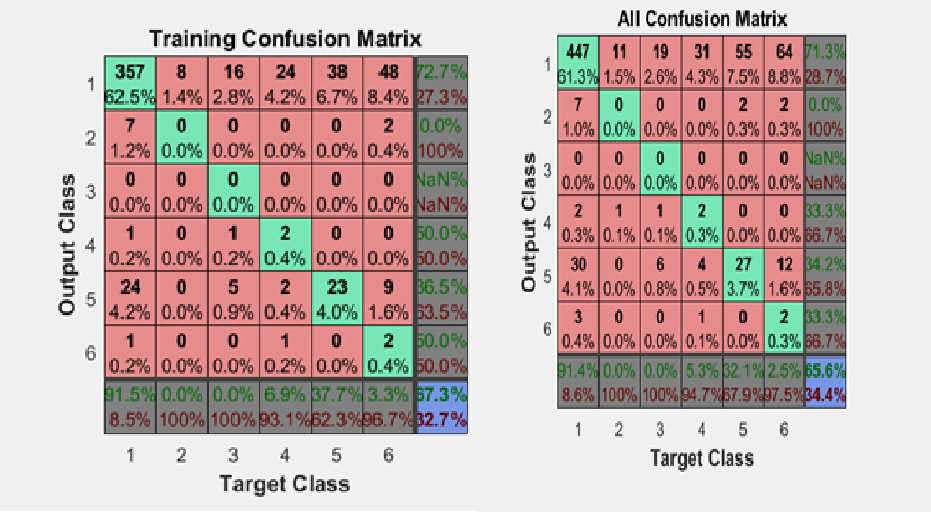
\includegraphics [scale=0.7]{result5.png}
\end{figure}
The input given Below is the table that shows the combination of methods we tried and their result.
\begin{figure}[H]
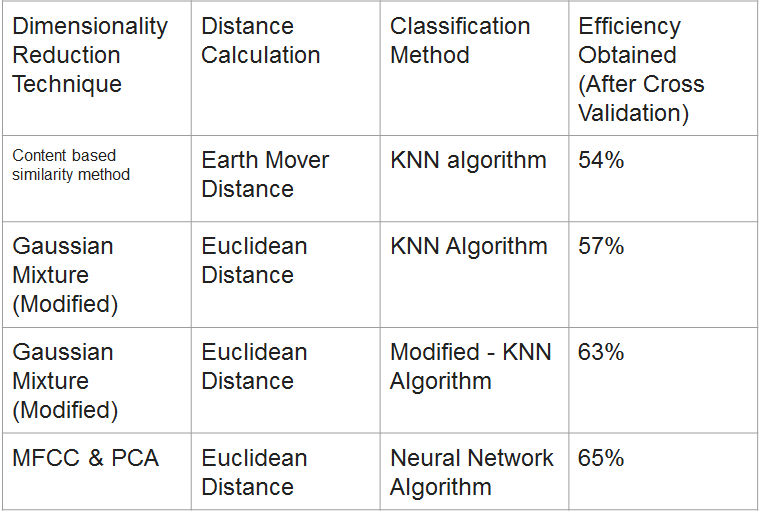
\includegraphics [scale=0.7]{table.png}
\end{figure}
%_________________________________________________________________
\section{Discussion}\label{sec:disc}
Music genre classification is a hard task. Our approach is three fold: Apply dimension reduction, calculate distance matrix and classify the data into its corresponding genres. For each stage, we experimented with different algorithms in an effort to achieve better accuracy across individual genres as well as overall accuracy.One of the important challenge that we encountered was the distribution of the data. The dataset has proportionately more classical songs than the other genres such as jazz or rock pop. This bias led to higher accuracy in classical and bad performance across another genres. As a solution we tried implementing modified k-nearest neighbours. Although, the accuracy improved from 57$\%$ to 63$\%$, the accuracy across classical dropped while the accuracy increased across other genres.

\paragraph{}
As the next steps, we would like to try extracting features such as rythm, modulation, amplification and other parameters instead of just the raw signal \cite{tzan} \cite{lee}. In addition, we are interested in studying the performance of the algorithm across different possible distance metrics. For example: In content based similarity dimensionality reduction, we use k-Means along with euclidean distance to cluster. How would it differ if we used Kullback Leibler instead of euclidean?. With respect of neural networks we would like to try different learning algorithms such as particle swarm optimization in order to find the synaptic weights of the network \cite{gudise}. Overall, the next steps would focus on improving the accuracy across genres as well as the overall accuracy.
\begin{thebibliography}{9}
	\bibitem{logan}\label{logan}
	Logan, B., & Salomon, A. (2001). A content-based music similarity function. Cambridge Research Labs-Tech Report.
	\bibitem{pampalk}\label{pampalk}
	Pampalk, E. (2006). Computational models of music similarity and their application in music information retrieval. na.
	\bibitem{lee}
	Lee, C. H., Shih, J. L., Yu, K. M., & Lin, H. S. (2009). Automatic music genre classification based on modulation spectral analysis of spectral and cepstral features. IEEE Transactions on Multimedia, 11(4), 670-682.
	\bibitem{tzan}
	Tzanetakis, George, and Perry Cook. "Musical genre classification of audio signals." IEEE Transactions on speech and audio processing 10.5 (2002): 293-302.
	\bibitem{holand}
	Holand, S. M. (2008). Principal components analysis (PCA). Department of Geology, University of Georgia, Athens, GA.
	\bibitem{logmfcc}
	Logan, B. (2000, October). Mel Frequency Cepstral Coefficients for Music Modeling. In ISMIR.
	\bibitem{li}
	Li, T., Ogihara, M., & Li, Q. (2003, July). A comparative study on content-based music genre classification. In Proceedings of the 26th annual international ACM SIGIR conference on Research and development in informaion retrieval (pp. 282-289). ACM.
	\bibitem{dasgupta}
	Dasgupta, S., & Gupta, A. (2003). An elementary proof of a theorem of Johnson and Lindenstrauss. Random Structures & Algorithms, 22(1), 60-65.
	\bibitem{gudise}
	Gudise, V. G., & Venayagamoorthy, G. K. (2003, April). Comparison of particle swarm optimization and backpropagation as training algorithms for neural networks. In Swarm Intelligence Symposium, 2003. SIS'03. Proceedings of the 2003 IEEE (pp. 110-117). IEEE.
\end{thebibliography}
\end{document}